\section{Method}
    
    %Describe your the sample and if applicable its growth method \\ \\
    %CrSb (chromium antimonide) (made with sputtering? Sample was acquired from elsewhere, need to enquire about what method was actually used.)
    %2.5x2 mm \\ \\
    %Measured in a PPMS(Physical Property Measurement System). First at constant magnetic field of 1 T with varying temperature 5-300 K \\ \\
    %Describe the magnetization measurements. \\ \\ The sample was acquired from [I DON'T KNOW]. 
    All measurements were made using a Physical Property Measurement System (PPMS) which allows one to measure the magnetization of a sample both as a function of temperature and as a function of the applied external magnetic field. The PPMS contains a sample holder which may oscillate up and down at a frequency of 40 Hz with an amplitude of 1-3 mm. This oscillation causes a change in the magnetic field generated by the sample, meaning a voltage is induced in a nearby detection coil. The PPMS also contains coils used for generating magnetic fields that can reach large magnitudes \cite{ppmsmanual}.
    \begin{figure}
    \centering
    \includegraphics[width=0.7\linewidth]{images/ppms_image.jpg}
    \caption{PPMS used for measurements. Made by Quantum Design \cite{ppmsmanual}.}
    \label{fig:ppms-image}
\end{figure}
    \subsection{Magnetization vs. Temperature}
    The sample was cut into a block of dimensions 0.15 × 0.08 × 0.01cm³.
    It was then attached to the sample holder, using varnish, at an offset of as near 35 mm as possible. The sample holder was put into the PPMS and an automatic centering routine was performed. A macro was created which instructed the PPMS to first lower its temperature to 5 K without any magnetic field and only afterwards applying a 1 T magnetic field in order to measure the Zero Field Cooled (ZFC) properties. The temperature was then slowly raised while measurements of the magnetization were performed until the temperature reached 300 K. After reaching 300 K, the temperature was dropped to 5 K again, this time with the magnetic field active during the cooling in order to perform Field Cooled (FC) measurements. After reaching 5 K, the temperature was slowly raised back to 300 K while measurements were made and the data saved. After the first experiment, the experiment was repetead, but with the sample rotated by 90\degree \hspace{1pt} to measure the anisotropic effects. The first position was denoted the a-axis and the second was denoted the b-axis. A third experiment was done with the sample position changed to have it perpendicular to the front of the sample in experiments one and two, as seen in \autoref{fig:both-samples}.
    %[SHOULD MORE DETAILS BE PROVIDED, EG. WAIT TIMES FOR STABILIZATION]
    \begin{figure}
    \centering
    \begin{subfigure}{0.45\textwidth}
        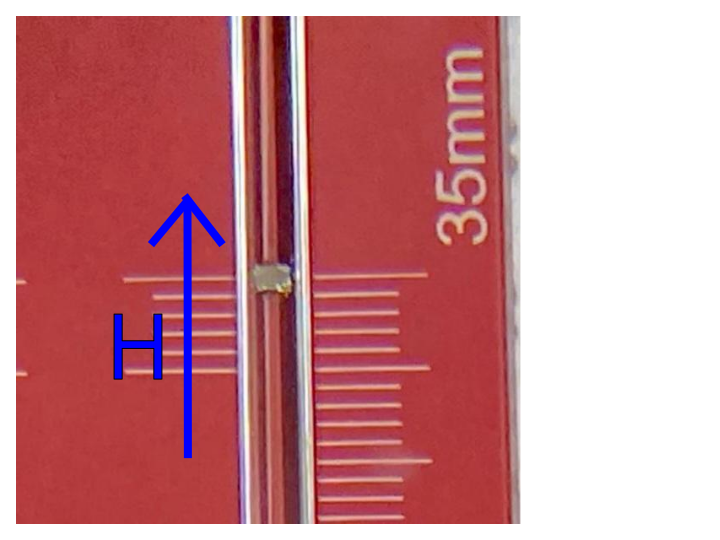
\includegraphics[width=1.4\linewidth]{pdf_files/sample_a_arrow.pdf}
        \caption{First position of sample, with the magnetic field along the a-axis.}
        \label{fig:original-sample}
    \end{subfigure} \hfill
    \begin{subfigure}{0.45\textwidth}
        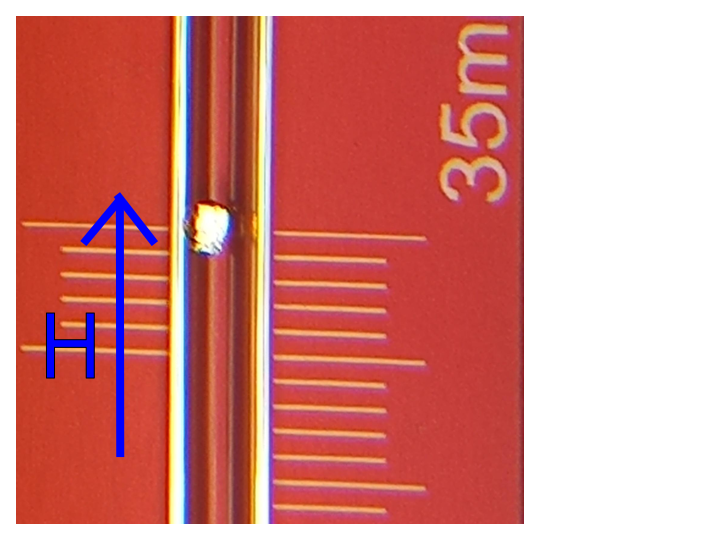
\includegraphics[width=1.4\linewidth]{pdf_files/sample_b_arrow.pdf}
        \caption{Second position of sample, with the magnetic field along the b-axis.}
        \label{fig:rotated-sample}
    \end{subfigure}
    \begin{subfigure}{0.45\textwidth}
        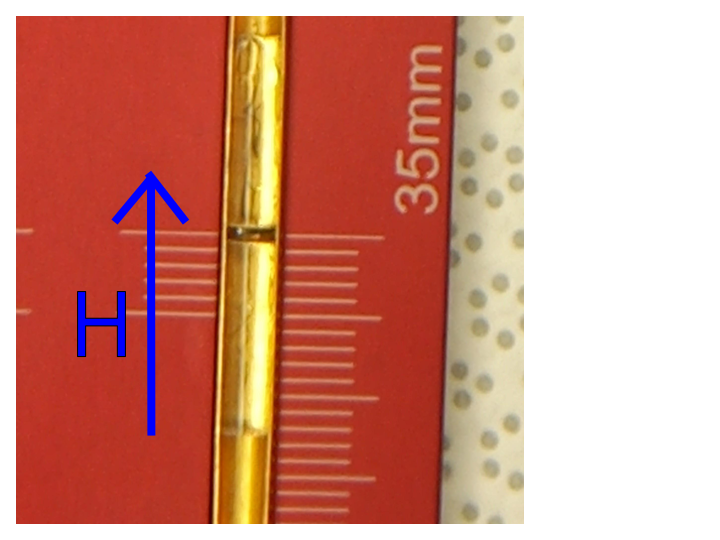
\includegraphics[width=1.4\linewidth]{pdf_files/sample_c_arrow.pdf}
        \caption{Third position of sample, with the magnetic field along the c-axis.}
        \label{fig:sample-pos-c}
    \end{subfigure}
    \caption{Sample mounted on holder before each M vs. T experiment. During each experiment, the magnetic field was going from the bottom to the top of the image, as shown by the blue arrows.}
    \label{fig:both-samples}
\end{figure}
    \subsection{Magnetization vs. Magnetic Field}
    The PPMS was mounted with a thin sample of CrSb with dimensions 0.15 × 0.08 × 0.01cm³. The PPMS was then activated at a temperature of 300 K and a magnetic field of 9 T. The magnetic field was then gradually lowered while the resulting magnetization of the sample was recorded. The magnetic field was lowered to 0 Tesla before being increased again, but in the opposite direction, which can also be thought of as a negative field. This field was increased/decreased all the way to -9 T, before once again changing direction and gradually reaching + 9 T again. The same procedure was repeated for the temperatures 100 K, 75 K, 50 K, 20 K and 5 K.

